\documentclass{article}
\usepackage[margin=2.5cm]{geometry}
\usepackage{graphicx}
\usepackage{listings}
\usepackage{xcolor}

\definecolor{codegreen}{rgb}{0,0.6,0}
\definecolor{codegray}{rgb}{0.5,0.5,0.5}
\definecolor{codepurple}{rgb}{0.58,0,0.82}
\definecolor{backcolour}{rgb}{0.95,0.95,0.92}

\lstdefinestyle{mystyle}{
    backgroundcolor=\color{backcolour},   
    commentstyle=\color{codegreen},
    keywordstyle=\color{magenta},
    numberstyle=\tiny\color{codegray},
    stringstyle=\color{codepurple},
    basicstyle=\ttfamily\footnotesize,
    breakatwhitespace=false,         
    breaklines=true,                 
    captionpos=b,                    
    keepspaces=true,                 
    numbers=left,                    
    numbersep=5pt,                  
    showspaces=false,                
    showstringspaces=false,
    showtabs=false,                  
    tabsize=2
}

\lstset{style=mystyle}

\begin{document}

\title{\LARGE \textbf{Protokol o semestrálním projektu z předmětu Elektronika a komunikace}\\{\Large Zpracování dat z IMU}}
\author{Macháček Tomáš}

\maketitle

\vspace{2em}

\section{Popis zapojení}

Senzor inerciálních veličin MPU9250 (dále IMU) je připojen čtyřmi vodiči k vývojovému kitu ESP32. Dva slouží k napájení IMU (poskytováno kitem) a ostatní dva pro přenos dat po sběrnici I2C. Deska je napájena USB kabelem a zároveň je přes něj řešen přenos dat mezi ESP a počítačem.

\section{Schéma zapojení}

\begin{center}
    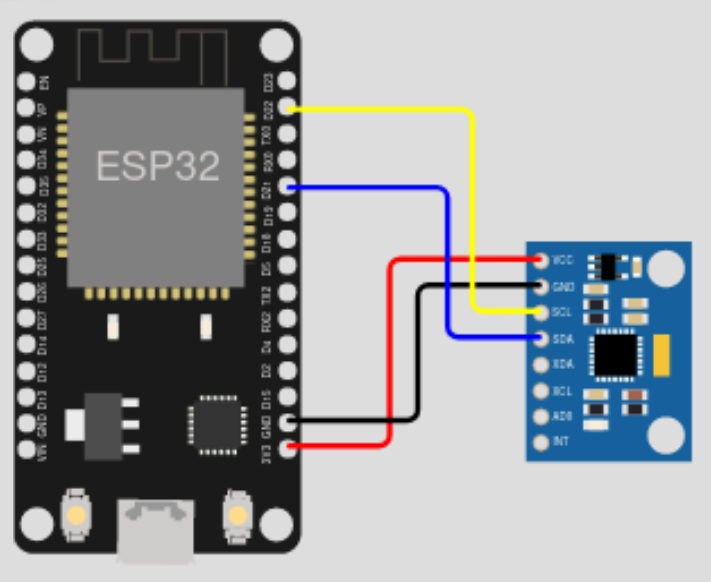
\includegraphics[width=10cm]{scheme.png}
\end{center}

\newpage

\section{Popis kódu - ESP32}

\lstset{language=C++}
\lstinputlisting{../board/board.ino}

\vspace{1em}

Program slouží pouze k inicializaci senzoru MPU9250, periodickému záznamu dat z IMU a jejich následnému odeslání po sériavé lince do počítače (sběrnice UART).

\newpage

\section{Popis kódu na počítači}

Na počítači probíhá záznam (uložení) a zpracování dat. V souboru $board.conf$  se definují parametry sériové komunikace (musí být shodné s těma na ESP). Po spuštění programu se inicializuje sériový port podle konfiguračního souboru (pakliže se nastavení v souboru neuvede, nastaví se na základní hodnotu), poté se spustí záchyt dat. Po uplynutí časové konstanty (opět se dá nastavit v konfiguračním souboru), se mohou data buď uložit či zahodit. Data se ukládají do složky $data$ do souboru $output.csv$. Dále se mohou zpracovat prostřednicvím skriptu v pythonu, který vygeneruje grafy (nezpracované hodnoty, Eulerovy úhly, zrychlení, rychlost, pozici ve složkách a ve 3D). Výstupem je pdf soubor obsahující všechny grafy.

\subsection{Obsluha sériového portu}

Prostřednicvím rozhraní knihovny termios2 jsou nakonfigurovány parametry sériového portu. Jedná se o počet bitů v jednom rámci, paritní bit, počet stop bitů, baud rate, timeout, echo.

\subsection{Skript ke zpracování dat}

Pomocí knihovny matplotlib jsou vytvářeny všechny grafy, tím prvním je reprezentace dat vyčtených z IMU. 
Prostřednictvím Madgwickova filtru jsou hodnoty zpracovány do Eulerových úhlů (další graf). Dále je vytvořen graf akcelerace. Kvůli odstínění šumu ze senzoru bylo nutné zakomponovat do skriptu detektor pohybu, který rozhoduje zda je senzor v pohybu, či ne. Takto ošetřená data se mohou dále převést na rychlost jednoduchým vzorcem.

\begin{center}
    \begin{math}
        v = v_{0} + a \cdot \Delta t
    \end{math}
\end{center}

Rychlost je zobrazena složkově v grafu. Je převedena na graf zobrazující polohu po složkách.

\begin{center}
    \begin{math}
        s = s_{0} + v \cdot \Delta t
    \end{math}
\end{center}

Poloha je zanesena do grafu a poté je vizualizovaná 3D grafem.

\section{Možnosti, návrhy na zlepšení}

IMU bylo testováno ve všech třech směrech, přičemž chyba byla v řádech centimetrů. Délka záznamu byla pokaždé pět vteřín, při delším záznamu by se výrazně projevil drift oproti skutečné poloze. Řešením by byl kvalitnější senzor vybavený magnetometrem.

\section{Závěr}

Cílem projektu bylo zjistit možnosti levného IMU. 

\end{document}
